\subsection{User interfaces}
The interface of MyTaxiService can be for web application and mobile application. Here will be presented some of the most important pages and screens of MyTaxiService.

\paragraph{Log in:}
	In the figure below is shown the MyTaxiService's homepage
	\begin{center}
		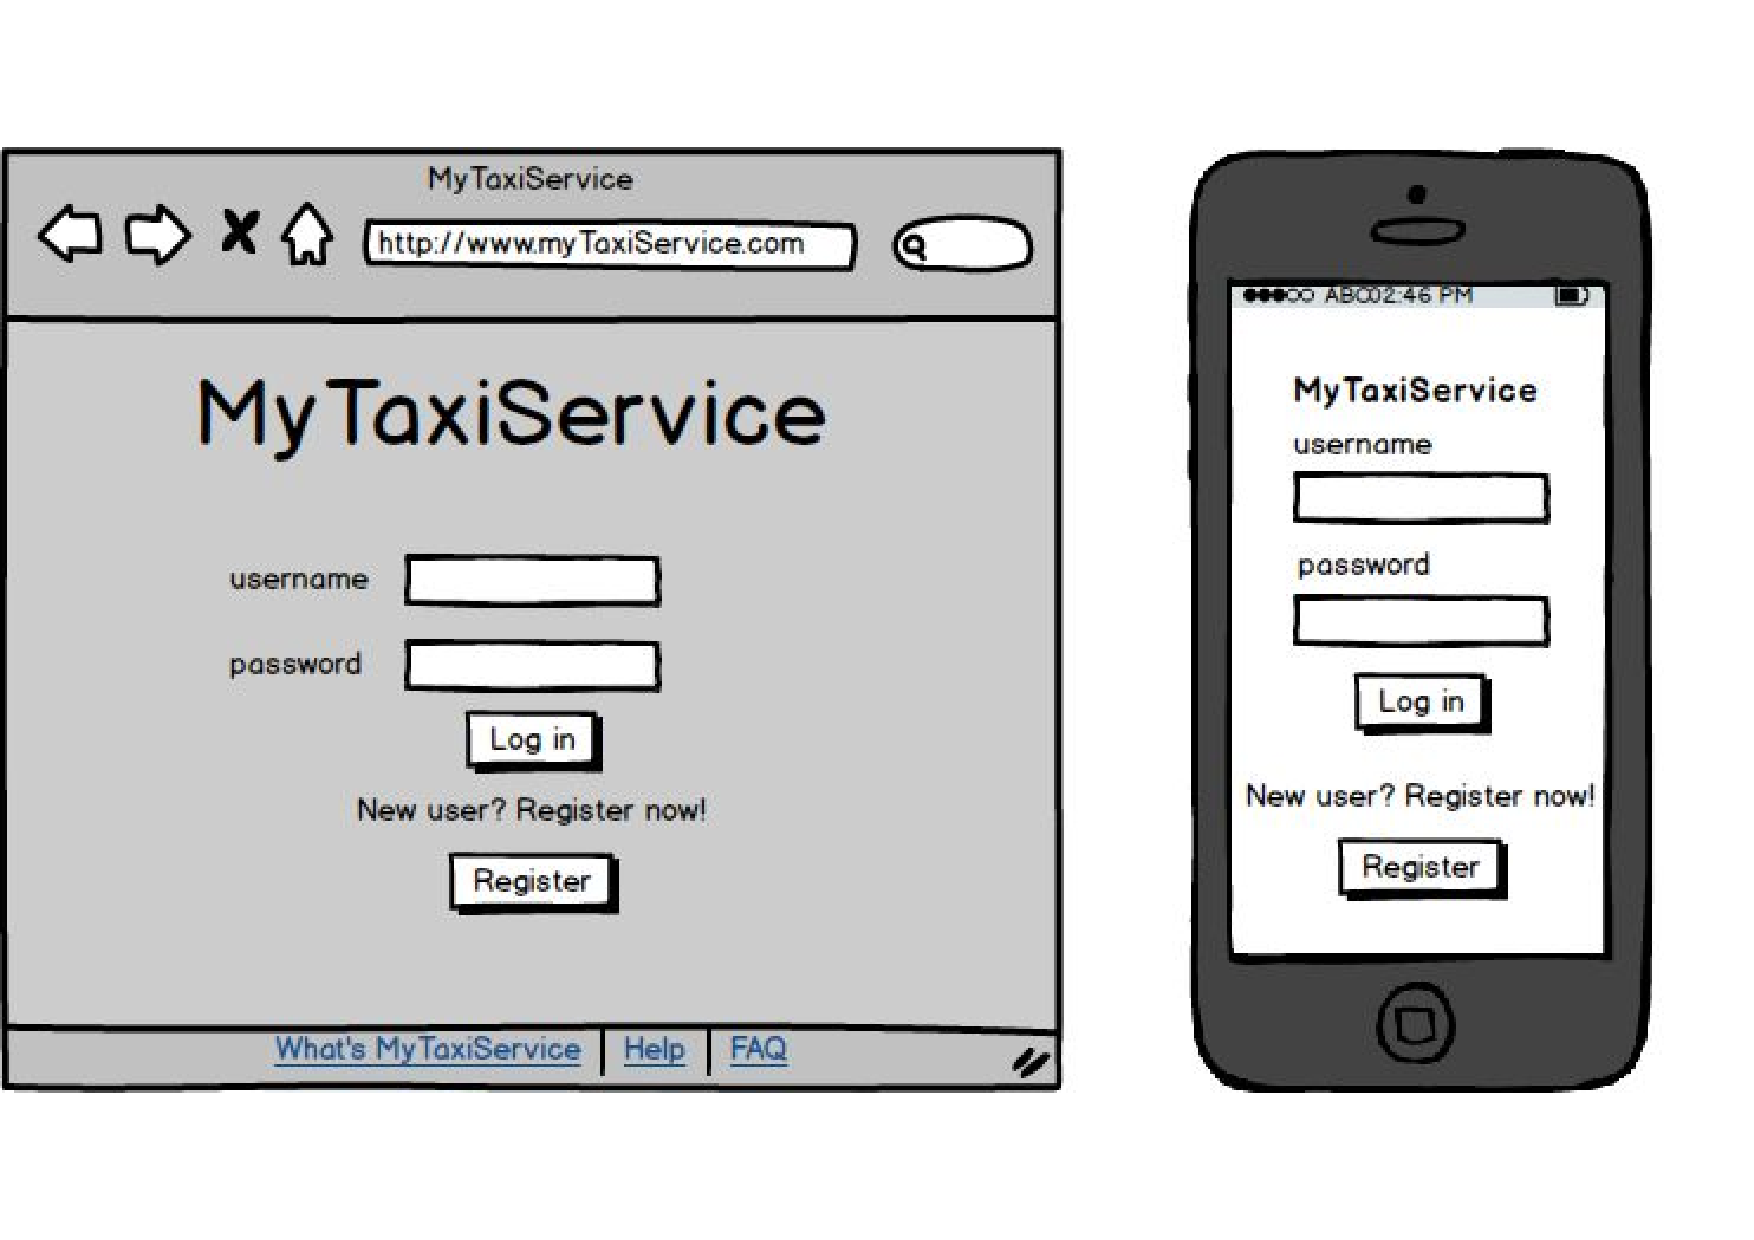
\includegraphics[width=\textwidth]{mockup/login.pdf}
	\end{center}
	
\paragraph{Registration:}
	Here the visitor can sig up to the application
\begin{center}
	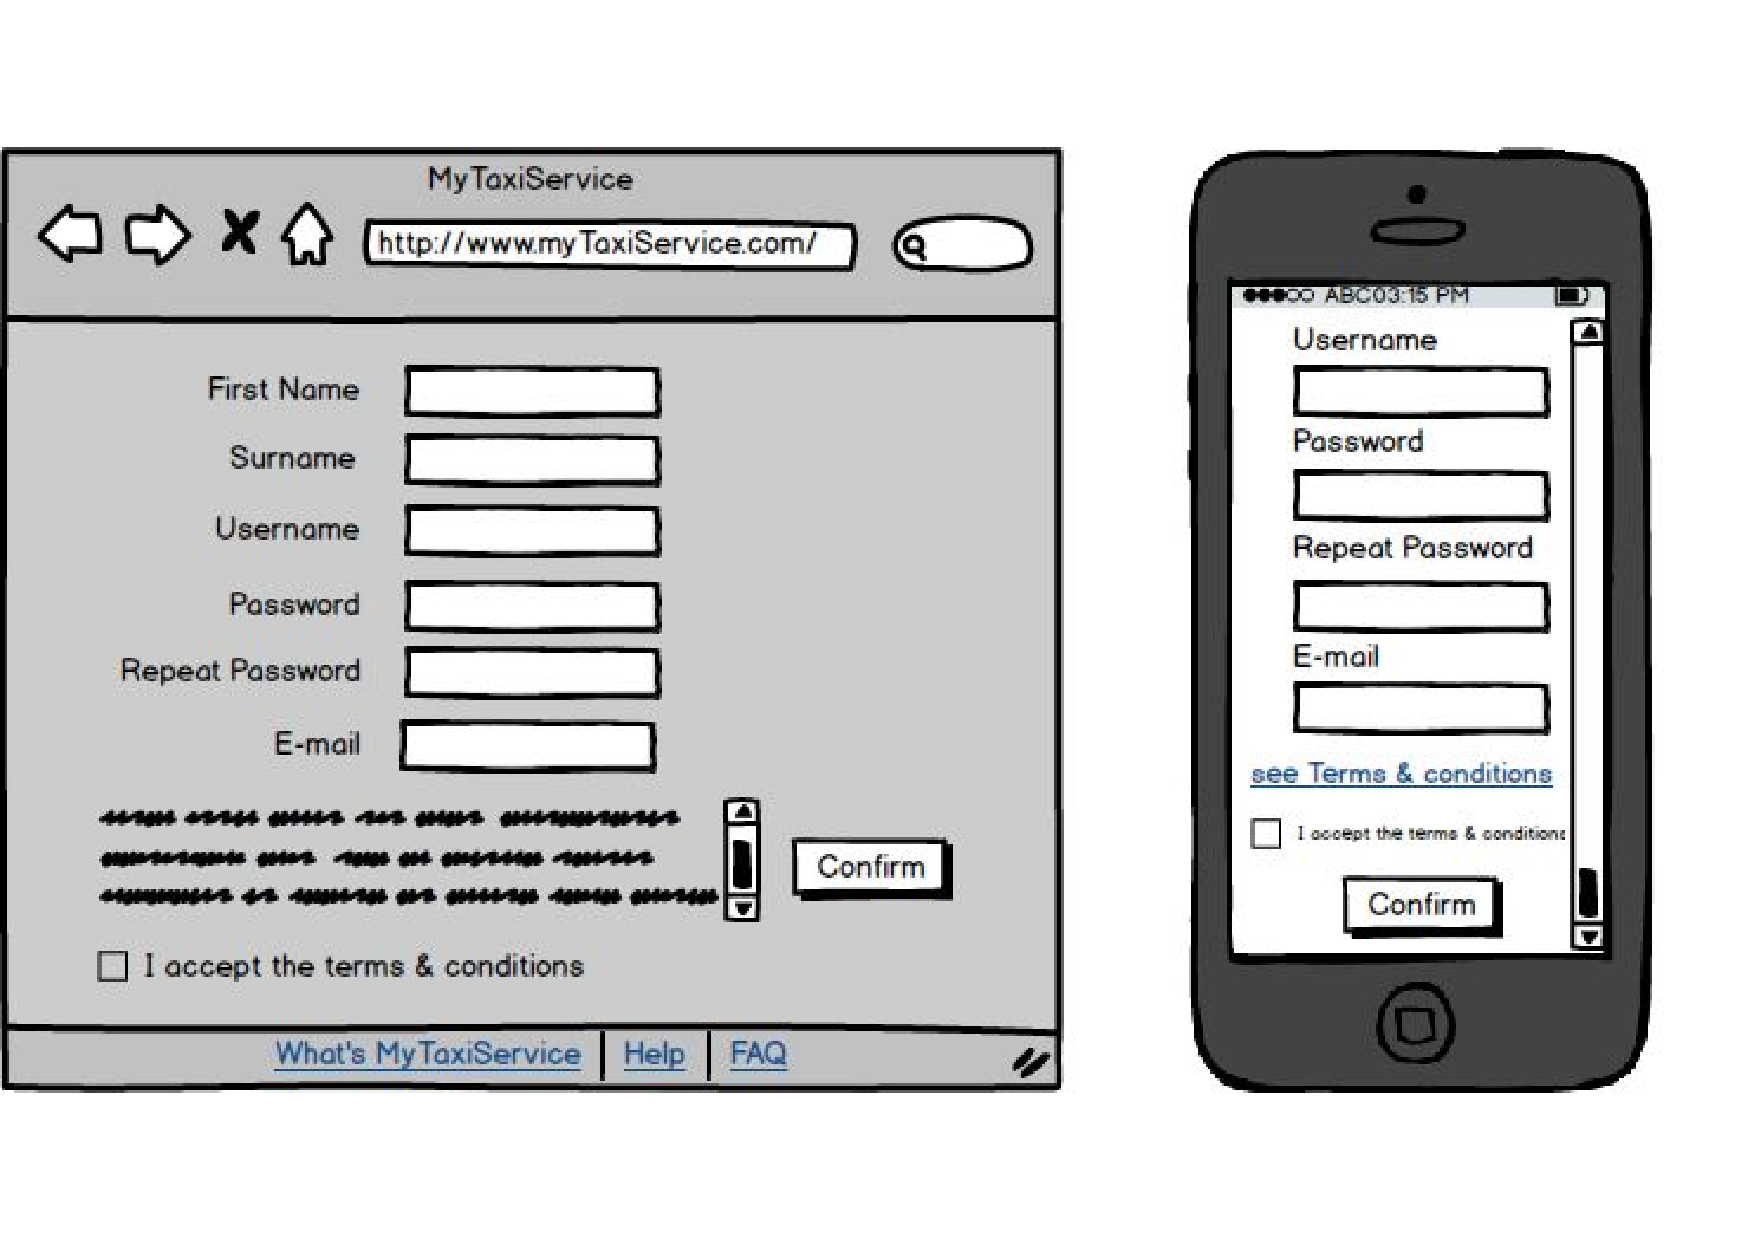
\includegraphics[width=\textwidth]{mockup/registration.pdf}
\end{center}

\paragraph{Passenger view:}
View of the passenger
\begin{center}
	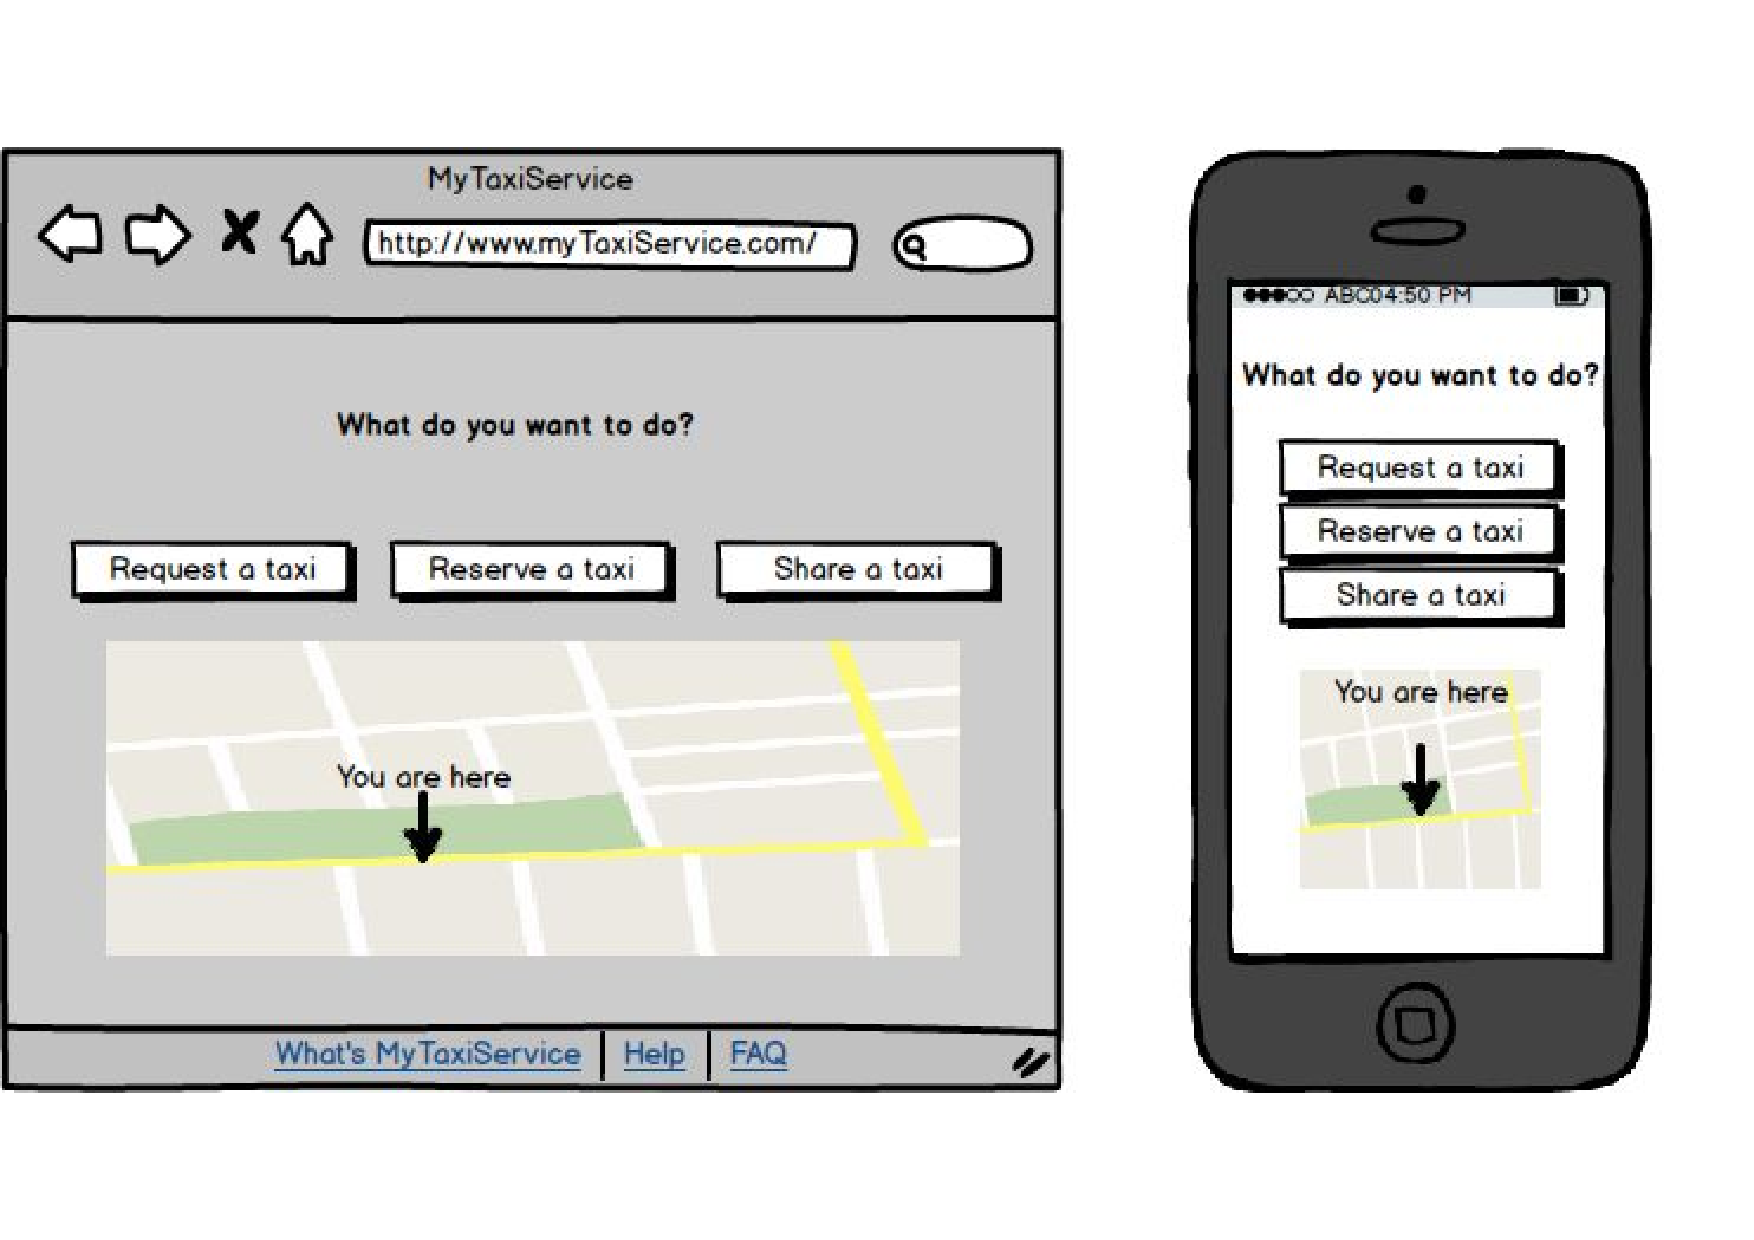
\includegraphics[width=\textwidth]{mockup/passengerFunctions.pdf}
\end{center}

\paragraph{Request a taxi:}
View of the passenger when he/she requests a taxi
\begin{center}
	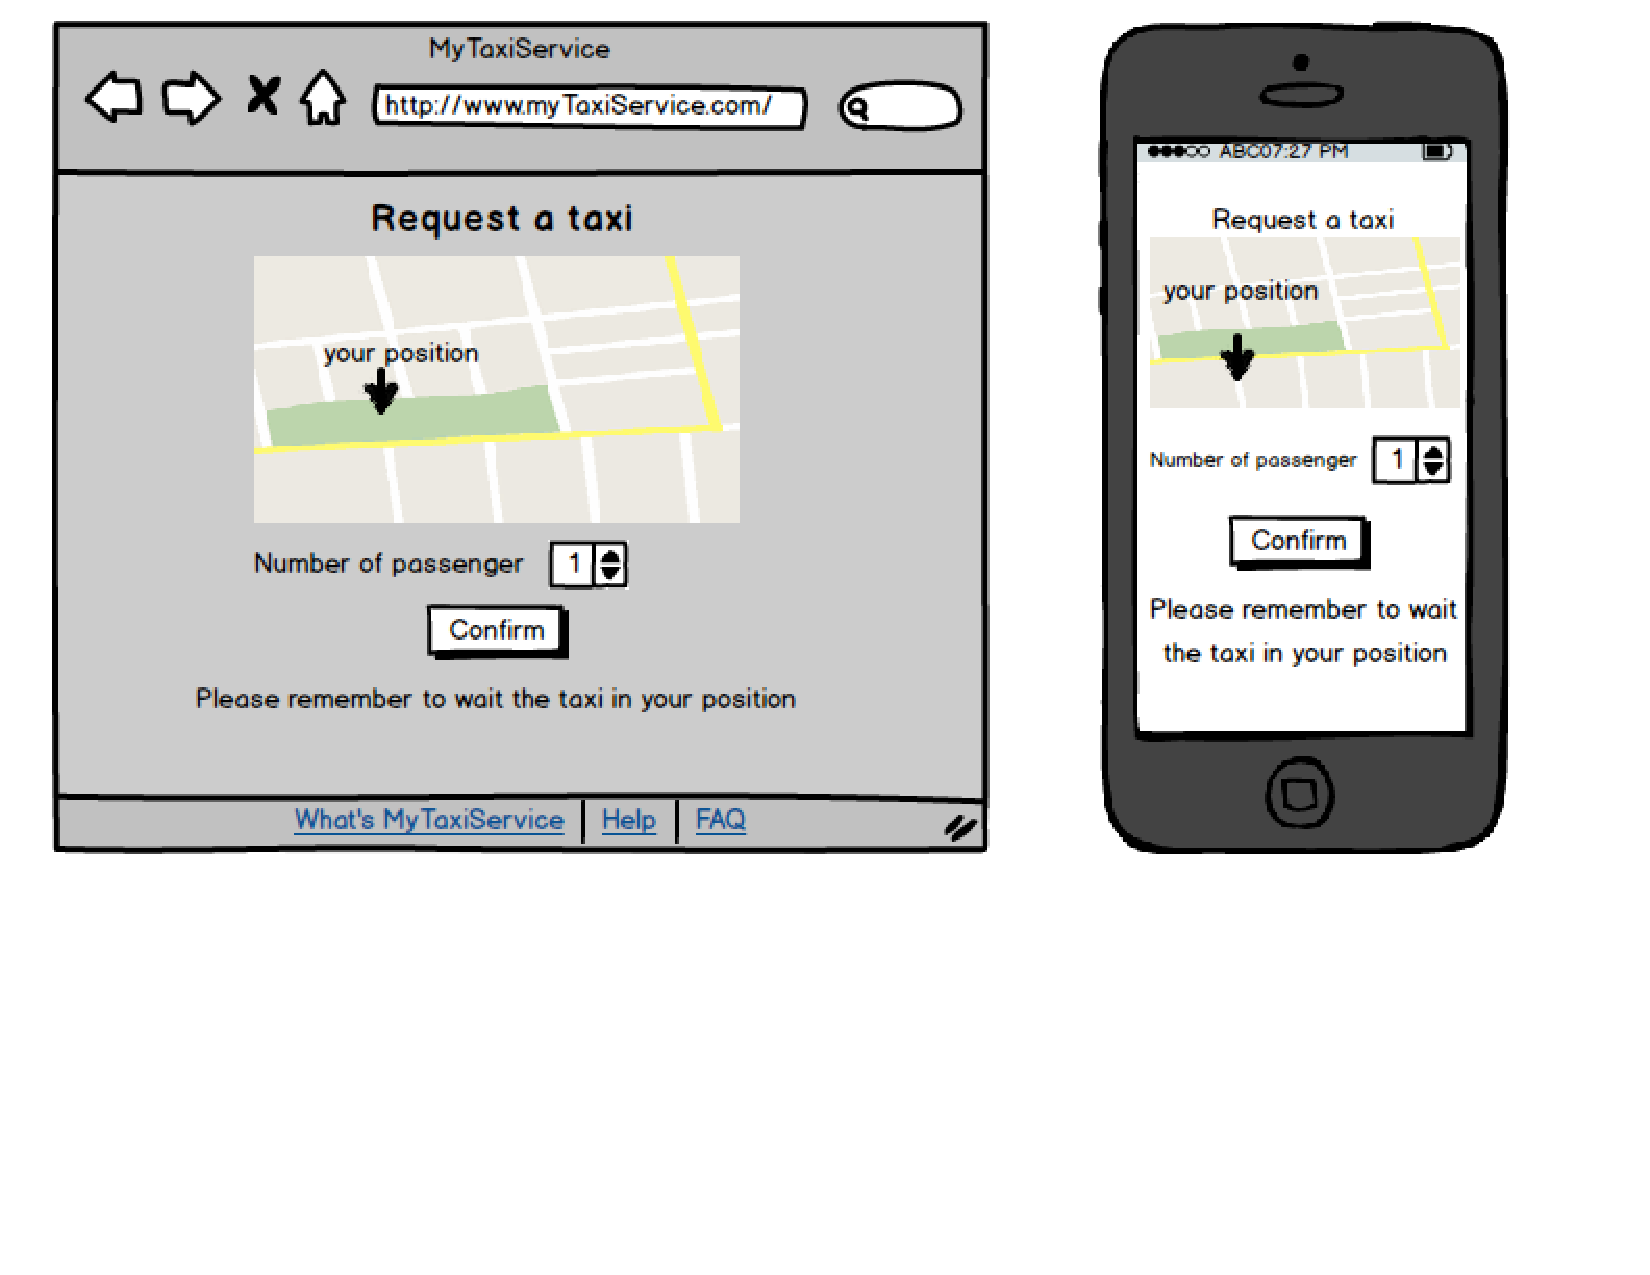
\includegraphics[width=\textwidth]{mockup/request.pdf}
\end{center}

\paragraph{Reserve a taxi:}
View of the passenger when he/she reserves a taxi
\begin{center}
	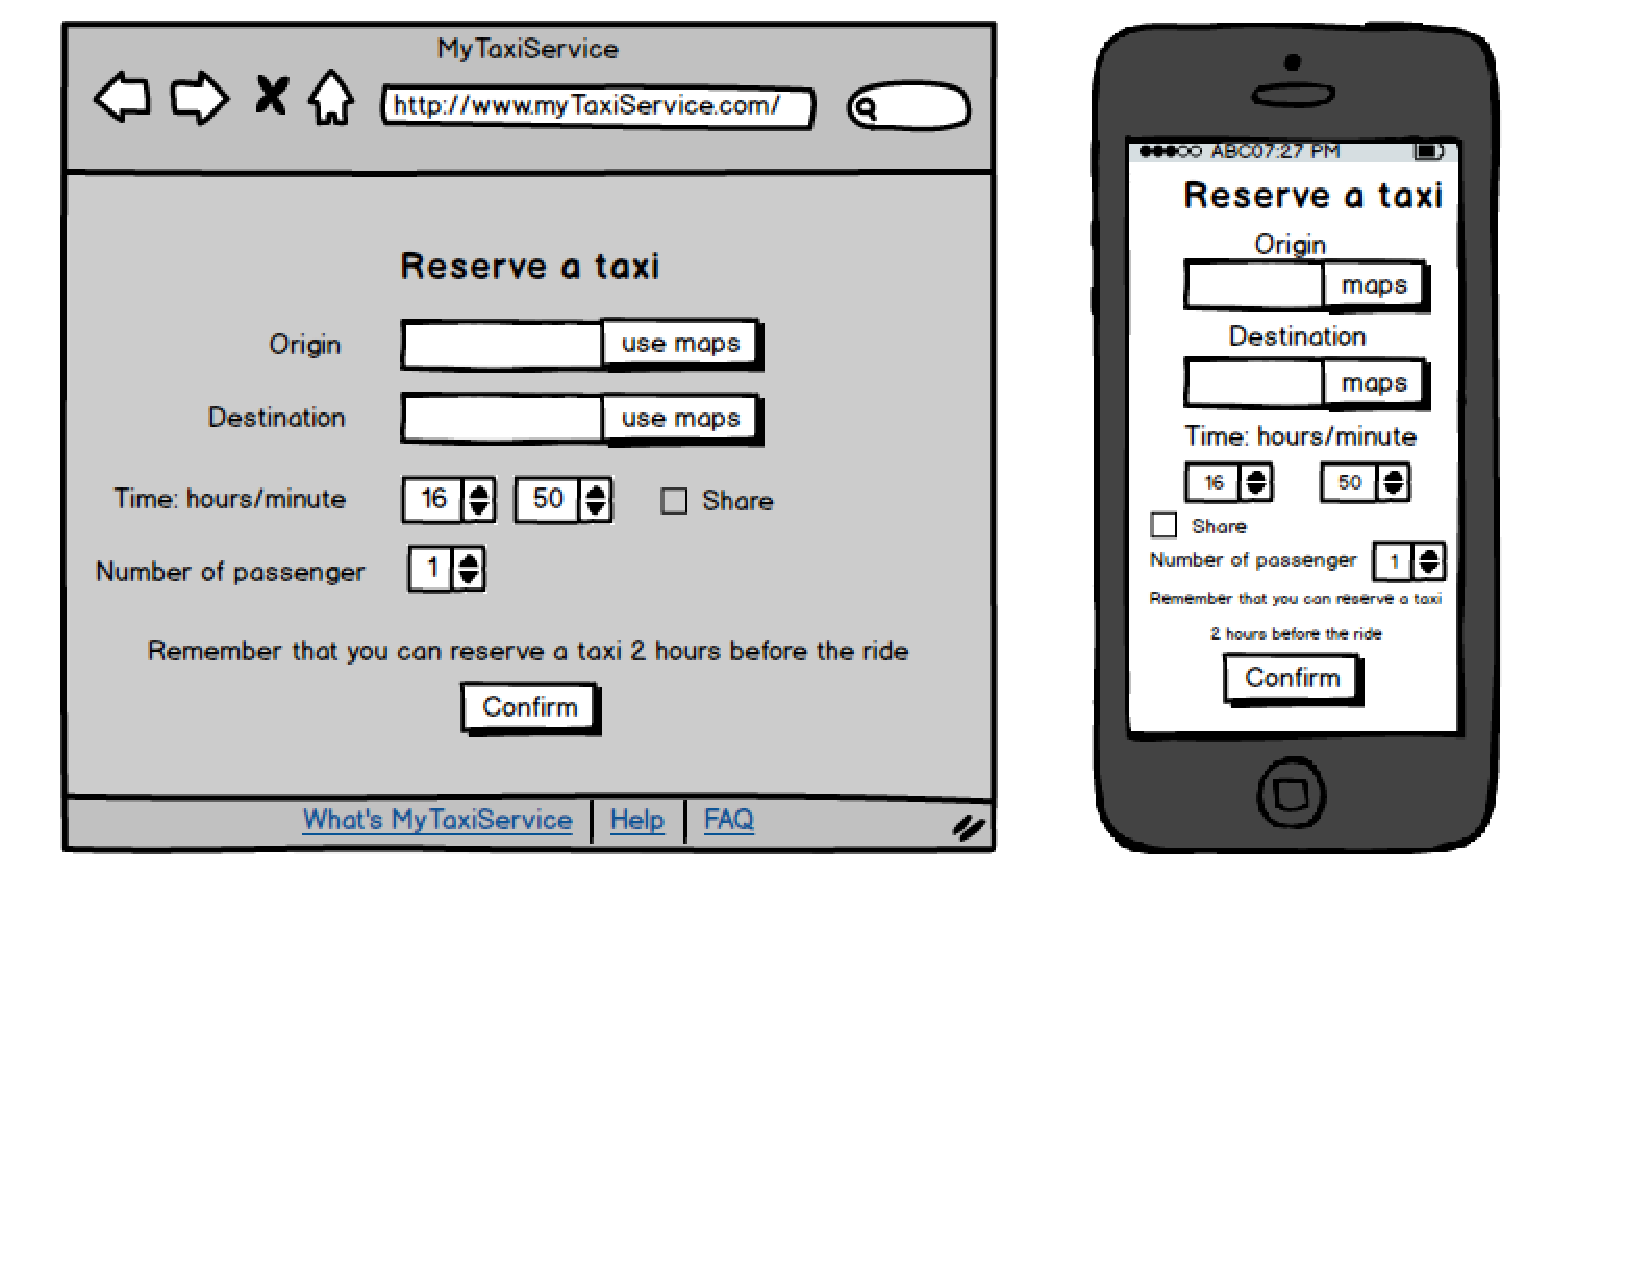
\includegraphics[width=\textwidth]{mockup/reserve.pdf}
\end{center}

\paragraph{Taxi driver view:}
View of the taxi driver
\begin{center}
	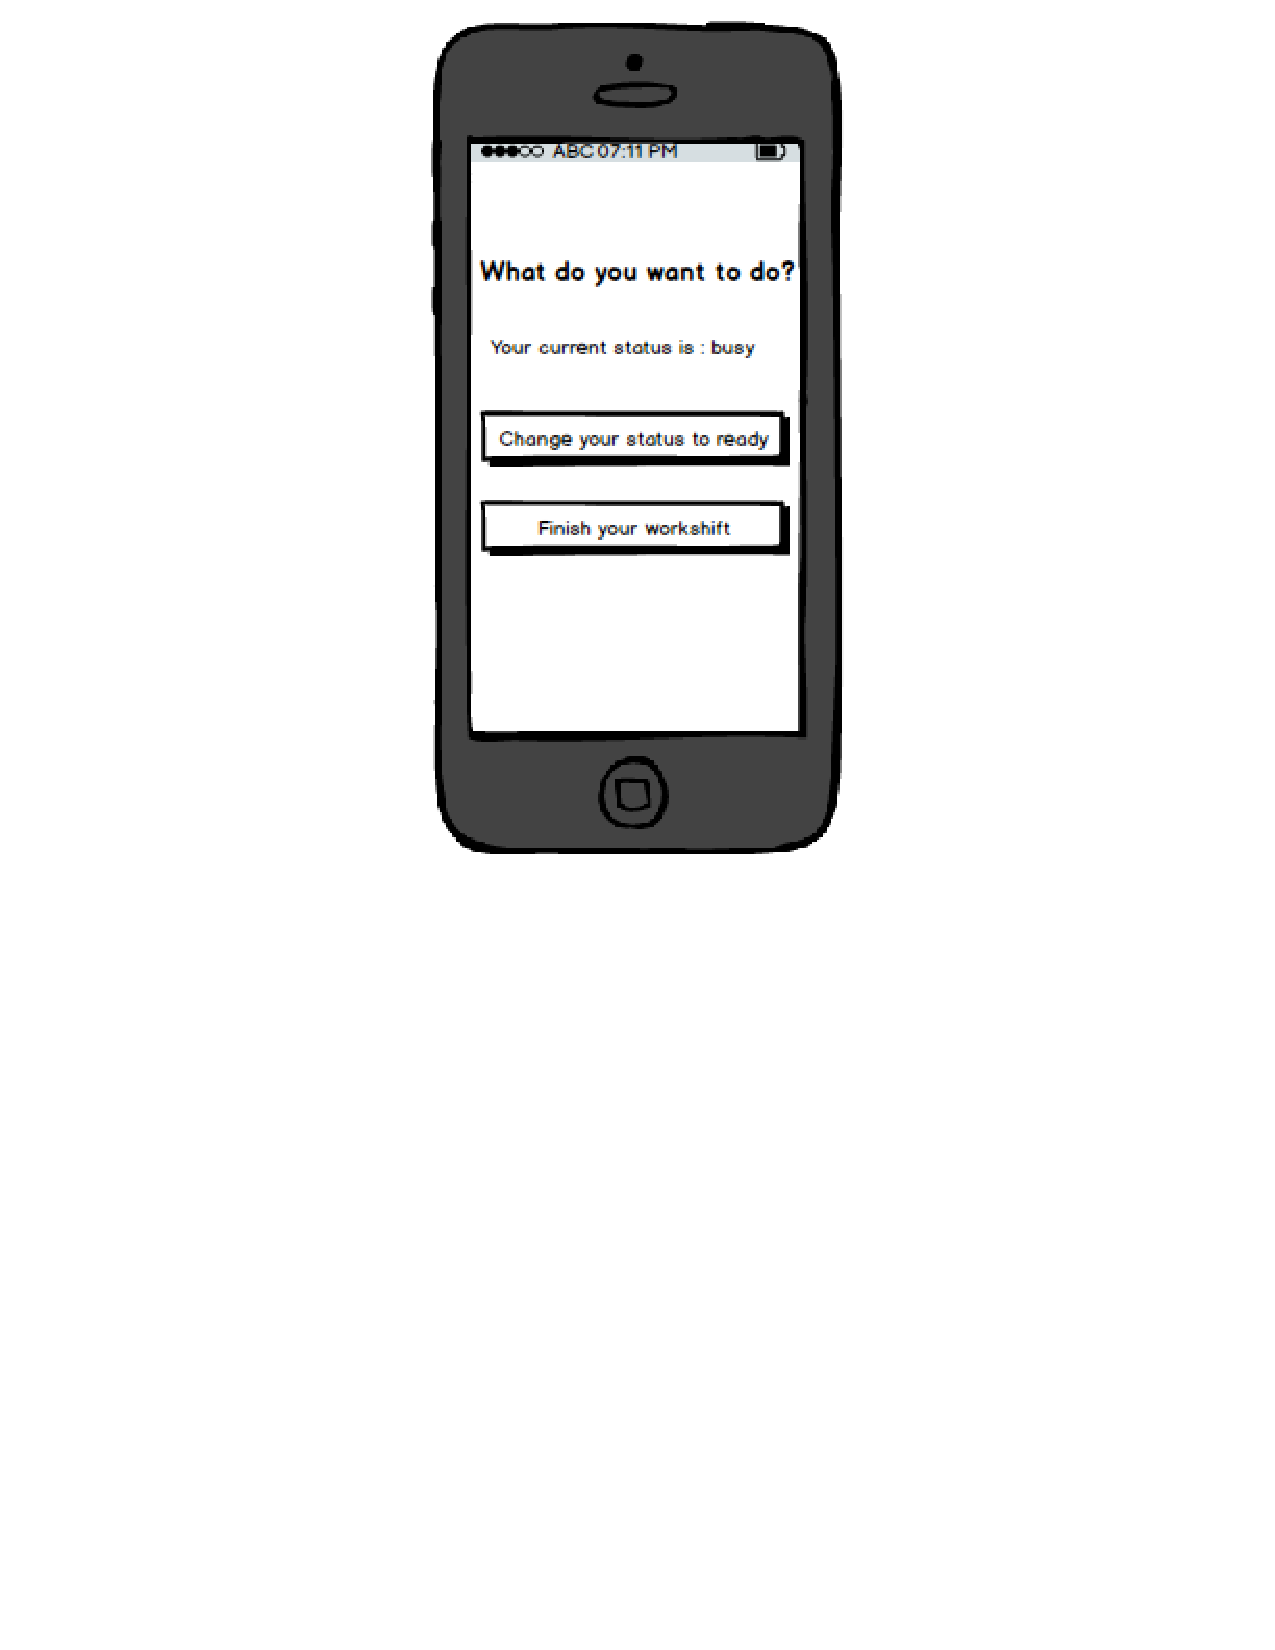
\includegraphics[width=\textwidth]{mockup/taxiDriverFunctions.pdf}
\end{center}

\paragraph{Taxi driver notification:}
Notification that the taxi driver, choosen by the system, sees when a passenger request a ride.
\begin{center}
	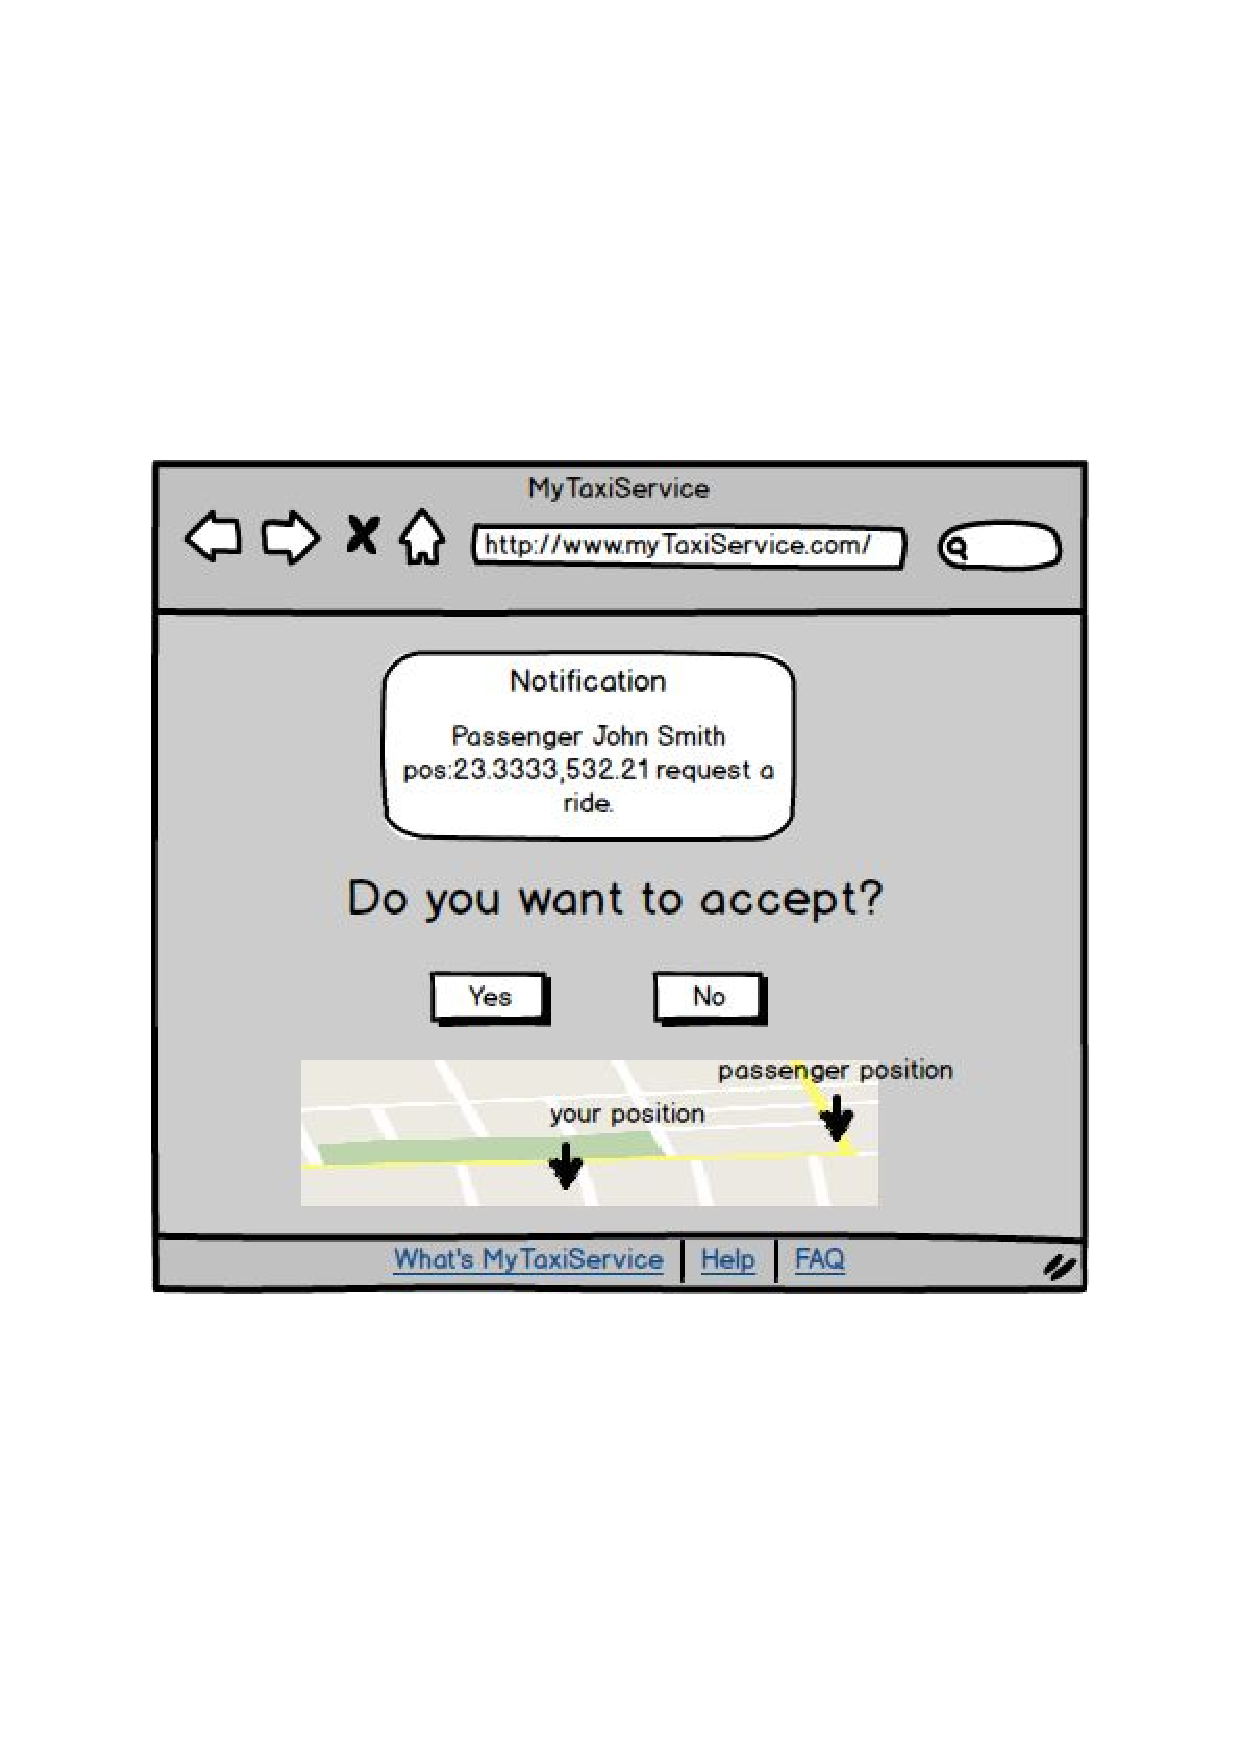
\includegraphics[width=\textwidth]{mockup/taxiDriverNotification.pdf}
\end{center}
\paragraph{Passenger notification :}
Notification that the passenger see when a taxi accept the ride
\begin{center}
	\includegraphics[width=\textwidth]{mockup/PassengerNotification.pdf}
\end{center}

\subsection{API interfaces}
MyTaxiService uses Google Maps APIs in order to show to the passengers and to the taxi driver their position in the city.
This API is continuos update and works for all the OS and browsers web supported by MyTaxiService.
More information are available on the site: https://developers.google.com/maps/

\subsection{Hardware interfaces}
MyTaxiService doesn't support any hardware interfaces.	\subsection{Software interfaces}
\begin{itemize}
	\item Database Management System (DBMS): \newline
	Name: MySQL \newline
	Version: 5.7 \newline
	Source: http://www.mysql.it/ 
	\item Java Virtual Machine (JVM):\newline
	Name: JEE \newline
	Version: 7 \newline
	Source: http://www.oracle.com/technetwork/java/javaee/tech/index.html
	\item Application server: \newline
	Name: Glassfish \newline
	Version: 4.1.1 \newline
	Source: https://glassfish.java.net/
\end{itemize}
\subsection{Communication interfaces}
\begin{itemize}
	\item Protocol: TCP Service: HTTPS Port : 443
	\item Protocol: TCP Service: HTTP  Port : 80
	\item Protocol: TCP Service: DBMS  Port : 9247
\end{itemize}
